\documentclass[12pt]{article}
\usepackage[pdfborder={0 0 0.5 [3 2]}]{hyperref}%
\usepackage[left=1in,right=1in,top=1in,bottom=1in]{geometry}%
\usepackage[shortalphabetic]{amsrefs}%
\usepackage{amsmath}
\usepackage{enumerate}
% \usepackage{enumitem}
\usepackage{amssymb}                
\usepackage{amsmath}                
\usepackage{amsfonts}
\usepackage{amsthm}
\usepackage{bbm}
\usepackage[table,xcdraw]{xcolor}
\usepackage{tikz}
\usepackage{float}
\usepackage{booktabs}
\usepackage{svg}
\usepackage{mathtools}
\usepackage{cool}
\usepackage{url}
\usepackage{graphicx,epsfig}
\usepackage{makecell}
\usepackage{array}

\def\noi{\noindent}
\def\T{{\mathbb T}}
\def\R{{\mathbb R}}
\def\N{{\mathbb N}}
\def\C{{\mathbb C}}
\def\Z{{\mathbb Z}}
\def\P{{\mathbb P}}
\def\E{{\mathbb E}}
\def\Q{\mathbb{Q}}
\def\ind{{\mathbb I}}

\DeclareMathOperator{\spn}{span}
\DeclareMathOperator{\ran}{range}

\graphicspath{ {suspension/} }

\newtheorem{lemma}{Lemma}
\newtheorem{theorem}{Theorem}
\newtheorem{corollary}{Corollary}
\newtheorem{definition}{Definition}
\newtheorem{assumption}{Assumption}
\newtheorem{hypothesis}{Hypothesis}

\newtheorem{notation}{Notation}

\begin{document}

\section{Suspension Bridge Equation}

\subsection{Background}

We look at the suspended beam equation from Chen97. The idea is to look at an equation which has a second order time derivative which also possesses multimodal solutions. This is suggested on p. 2095 of SanStrut and p. 351 of Chen97.\\

The equation we will look at is

\begin{equation}\label{susp}
u_{tt} + u_{xxxx} + e^{u - 1} - 1 = 0
\end{equation}

Note that the equation used for most of the analysis in Chen97 is 

\begin{equation}\label{susp2}
u_{tt} + u_{xxxx} + u^+ - 1 = 0
\end{equation}

which has a cusp at $u = 0$. On p. 351 of Chen97, Chen and McKenna note that they have proved existence of solutions only to \eqref{susp2}, not to \eqref{susp}, but there is strong numerical evidence that similar solutions exist for \eqref{susp}. At some point, we will look and see if this has been addressed. For now, we will say that the numerical evidence is ``good enough''.\\

We are interested in traveling wave solutions, so we take a modified form of the usual traveling wave ansatz. Letting $\xi = x - ct$, we take

\begin{equation}
u(x, t) = z(\xi, t) + 1 = z(x - ct, t) + 1
\end{equation}

Substituting this into \eqref{susp} gives us

\begin{equation*}
z_{tt} - c z_{\xi t} + c^2 z_{\xi \xi} + z_{\xi \xi \xi \xi} + e^{z} - 1 = 0
\end{equation*}

The advantage of adding 1 in our ansatz is that the background for $z$ is at $z = 0$, whereas for $u$ it is at $u = 1$. Since it's annoying to use $z$ and $\xi$, we rewrite this using $u$ and $x$ to get our traveling frame suspended beam equation

\begin{equation}\label{susp3}
u_{tt} - c u_{x t} + u_{xxxx} + c^2 u_{xx} + e^{u} - 1 = 0
\end{equation}

For an equilibrium solution (such as a homoclinic orbit), all time derivatives are zero, so any equilibrium solution must satisfy the ODE

\begin{equation}\label{eqODE}
u_{xxxx} + c^2 u_{xx} + e^{u} - 1 = 0
\end{equation}

which is (46) on p. 342 of Chen97, with $\tilde{f}(u) = e^u - 1$.\\

Note that $u = 0$ is a solution to this. A homoclinic orbit, if it exists, connects this trivial solution to itself. If we linearize about this trivial solution, we get the ODE

\begin{equation}
v_{xxxx} + c^2 v_{xx} + 1 = 0
\end{equation}

which has eigenvalues

\begin{equation}
\nu = \pm \sqrt{\frac{-c^2 \pm \sqrt{c^4 - 4}}{2} }
\end{equation}

Note that $\sqrt{c^4 - 4}$ is always less that $c^2$ is magnitude. If $|c| < \sqrt{2}$, we have a nice complex conjugate quartet $\nu = \pm \alpha \pm \beta i$. When $c = \sqrt{2}$, these eigenvalues collide on the imaginary axis at $\pm i$, then for $|c| > \sqrt{2}$ we have a quartet of purely imaginary eigenvalues. 

\subsection{Eigenvalue Problem}

For linear stability analysis, we look at the PDE eigenvalue problem. To do this, assume we have found an equilibrium solution $u^*(x)$ of \eqref{eqODE}. Then we linearize around this by taking the standard linearization ansatz

\begin{equation}
u(x,t) = u_*(x) + \epsilon e^{\lambda t} v(x)
\end{equation}

Plugging this into \eqref{susp3} and keeping only terms up to order $\epsilon$, we obtain the quadratic eigenvalue problem

\begin{equation}\label{evp}
[\lambda^2 - c \partial_x \lambda + (\partial_x^4 + c^2 \partial_x^2 + e^{u_*})]v = 0
\end{equation}

As far as I know, there is nothing out there on how to deal with this. So we have to figure that out.\\

First, let's write the eigenvalue problem as a first order system. Letting $V = (v_1, v_2, v_3, v_4) = (v, v_x, v_{xx}, v_{xxx})$, we have $V' = A(\lambda; u^*)V$, where

\begin{equation}
A(\lambda; u^*) = \begin{pmatrix}
0 & 1 & 0 & 0 \\
0 & 0 & 1 & 0 \\
0 & 0 & 0 & 1 \\
-(\lambda^2 + e^{u_*}) & c \lambda & -c^2 & 0 
\end{pmatrix}
\end{equation}

Assume we there exists an exponentially localized single pulse solution $u_0(x)$. Then, we can find the essential spectrum by looking at the asymptotic matrix

\begin{equation*}
A_\infty(\lambda) = \begin{pmatrix}
0 & 1 & 0 & 0 \\
0 & 0 & 1 & 0 \\
0 & 0 & 0 & 1 \\
-(\lambda^2 + 1) & c \lambda & -c^2 & 0 
\end{pmatrix}
\end{equation*}

The characteristic polynomial of this is 

\begin{equation}\label{charpoly}
p(\nu) = \nu^4 + c^2 \nu^2 - c \lambda \nu + (\lambda^2 + 1) 
\end{equation} 

For the essential spectrum, we want the values of $\lambda$ for which we have a purely imaginary eigenvalue, i.e. $\nu = i r$ for $r \in \R$. Plugging this in and collecting terms in $\lambda$, we get the equation

\begin{equation}\label{fredholmborder}
\lambda^2 - i c r \lambda - c^2 r^2  + r^4 + 1 = 0 
\end{equation} 

Solving for $\lambda$, we have

\begin{equation}
\lambda = \frac{1}{2} \left(i c r \pm 
\sqrt{3 c^2 r^2-4 r^4-4}\right)
\end{equation}

The term under the radical sign is a quadratic in $r^2$. Thus since $r^2 \geq 0$, the term under the radical sign has a maximum of $-4$ at $r = 0$ and decreases smoothly to $-\infty$ as $r^2 \rightarrow \infty$. From this we see that $\lambda$ is always pure imaginary. We can therefore write this as

\begin{equation}\label{lambdaimag}
\lambda(r) = \frac{1}{2} \left(c r \pm 
\sqrt{4 + 4 r^2 -3 c^2 r^2 }\right) i
\end{equation}

where all the stuff in front of the $i$ is real.\\

The next question is whether the essential spectrum is the entire imaginary axis. Mathematica suggests there is a gap in the essential spectrum around the origin, so let's try to find that.\\

The equation \eqref{lambdaimag} is of the form $\lambda_\pm(r) = k r \pm f(r^2)$. Since

\begin{align*}
\lambda_-(-r) = -kr - f((-r)^2) = -(kr + f(r^2)) = -\lambda_+(r)
\end{align*} 

it suffices to look at $\lambda_+(r)$. Using Mathematica, we find

\begin{align*}
\lambda_+'(r) = \frac{1}{2} \left(\frac{16 r^3-6 c^2 r}{2 \sqrt{4 r^4+4-3 c^2 r^2}}+c\right)
\end{align*}

Solving $\lambda_+'(r) = 0$ involves solving a 6th order polynomial, which Mathematica can do, but it is annoying so we won't deal with it for now. It appears that for $c > 0$, $\lambda_+'(r)$ has a minimum at some value $r_0$, and that $\lambda_+(r_0) > 0$. Thus numerical evidence suggests that essential spectrum has a gap around the origin. We will deal with this when we look at the numerics.

\subsection{Numerics}

The big issue here is that stationary solutions to \eqref{eqODE} are hard to come by. Nonetheless, we have figured out a way to compute these numerically, although it is a bit dicey. Our method is a variant of the mountain pass and string methods, and essentially combines Chen97 and Chamard10.

\begin{enumerate}
	\item The energy functional $I \in C^1(H^2, \R)$ is given by
	\begin{equation}
	I(z) = \frac{1}{2} \int_\R (|z''|^2 - c^2 |z'|^2)dx 
	+ \int_\R (e^z - z - 1) dx
	\end{equation}
	where $z$ is a function of $x$. For the numerical method, we truncate the domain to $[-L, L]$ for $L$ large.
	\item To do the mountain pass method, we need to find
	\begin{enumerate}
		\item A function $e_1 \in H^2$ which is a local minimum of $I$. From Lemma 2.4 in Chen97, $e_1 = 0$ satisfies this.
		\item A function $e_2 \in H^2$ for which $I(e_2) < I(e^1) = I(0) = 0$. We can use Lemma 2.5 in Chen97 to find such an $e_2$. 
	\end{enumerate} 
	The solution we want, by the Mountain Pass Lemma, is the infimum of the maxima of $I$ along all paths joining $e_1$ and $e_2$.
	\item Choose a discretization scheme. Following Chen97, we use the finite difference method.
	\item We then use the String Method from Chamard10.
	\begin{enumerate}
		\item Join $e_1$ and $e_2$ by a piecewise linear path $U(t) = t e_1 + (1-t) e_2 = (1-t)e_2$. Choose a discrete set of values for $t$ which are evenly spaced, i.e. the $N+1$ values $t = [0, 1/N, 2/N, ..., 1]$ for some reasonably sized $N$. We ended up using $N = 10$, which worked fine.
		\item Reparamaterize the path to get points more-or-less equidistantly distributed in the $H^1$ norm.
		\item Evaluate the steepest decent direction $v(t_i)$ for all points $U(t_i)$ along the path. The steepest descent direction is computed as in section 3 of Chen97.
		\item For constrained maximal step size $h_M$, perform gradient descent on all points on the path $U(t_i)$ in the direction of $v(t_i)$.
		\item Go back to the reparamaterization step, and repeat all this a bunch of times. Theoretically there is a termination condition, but we don't acutally need to worry about that since we will be using Matlab's \texttt{fsolve}.
	\end{enumerate}
	\item After doing this a bunch of times, take the element of the path for which $I(U(t_i))$ is maximum. Or take one close to the maximum. Use this as an initial guess for Matlab's \texttt{fsolve}. This should converge to the solution we are looking for.
	\item ????
	\item Profit
\end{enumerate}

Here are plots of the stationary solution $u(x)$ found using this method for $c = 1.354$ and $c = 1.40$. Compare these to figure 3 on p. 347 of Chen97. Note that by the substitution we performed, the baseline in our plots is at 0 as opposed to 1 in Chen97.

\begin{figure}[H]
\centering
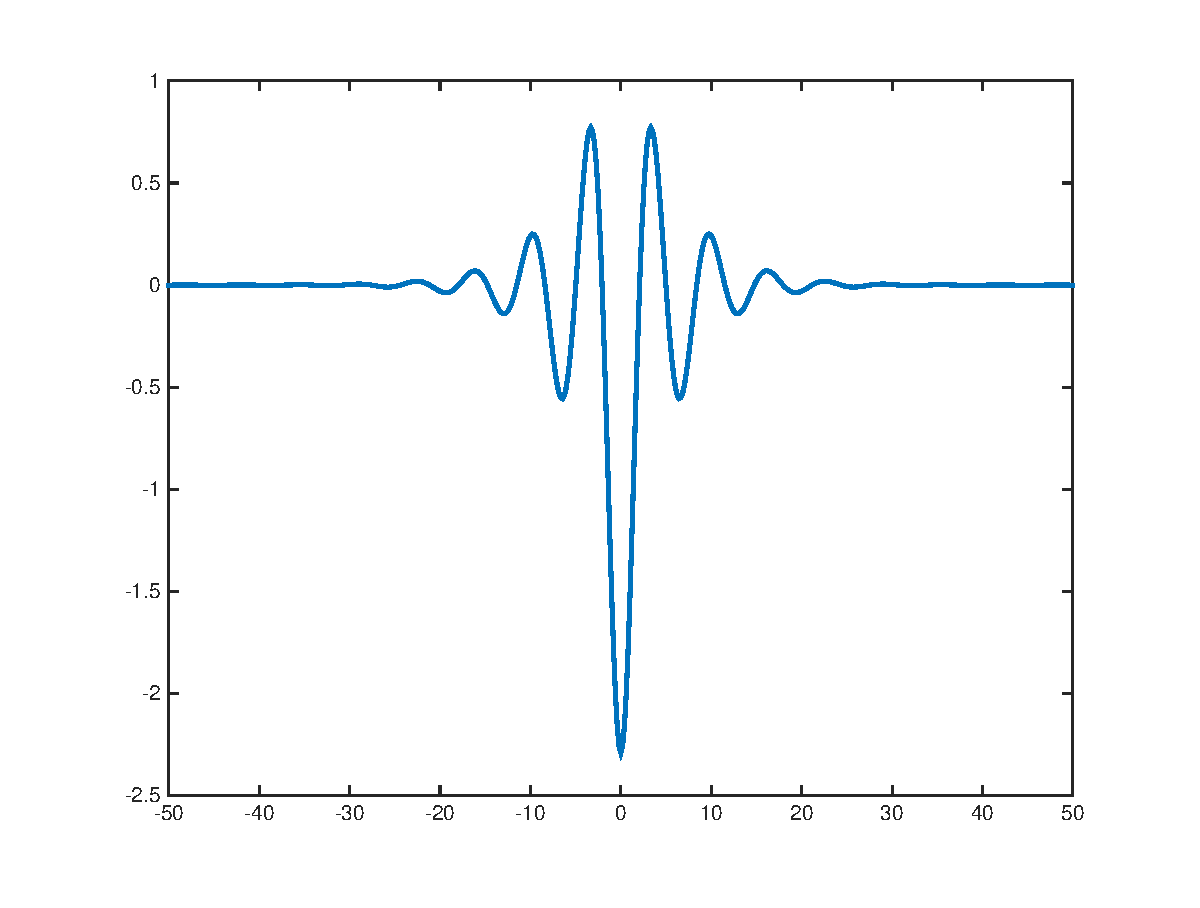
\includegraphics[width=8cm]{single1354.eps}
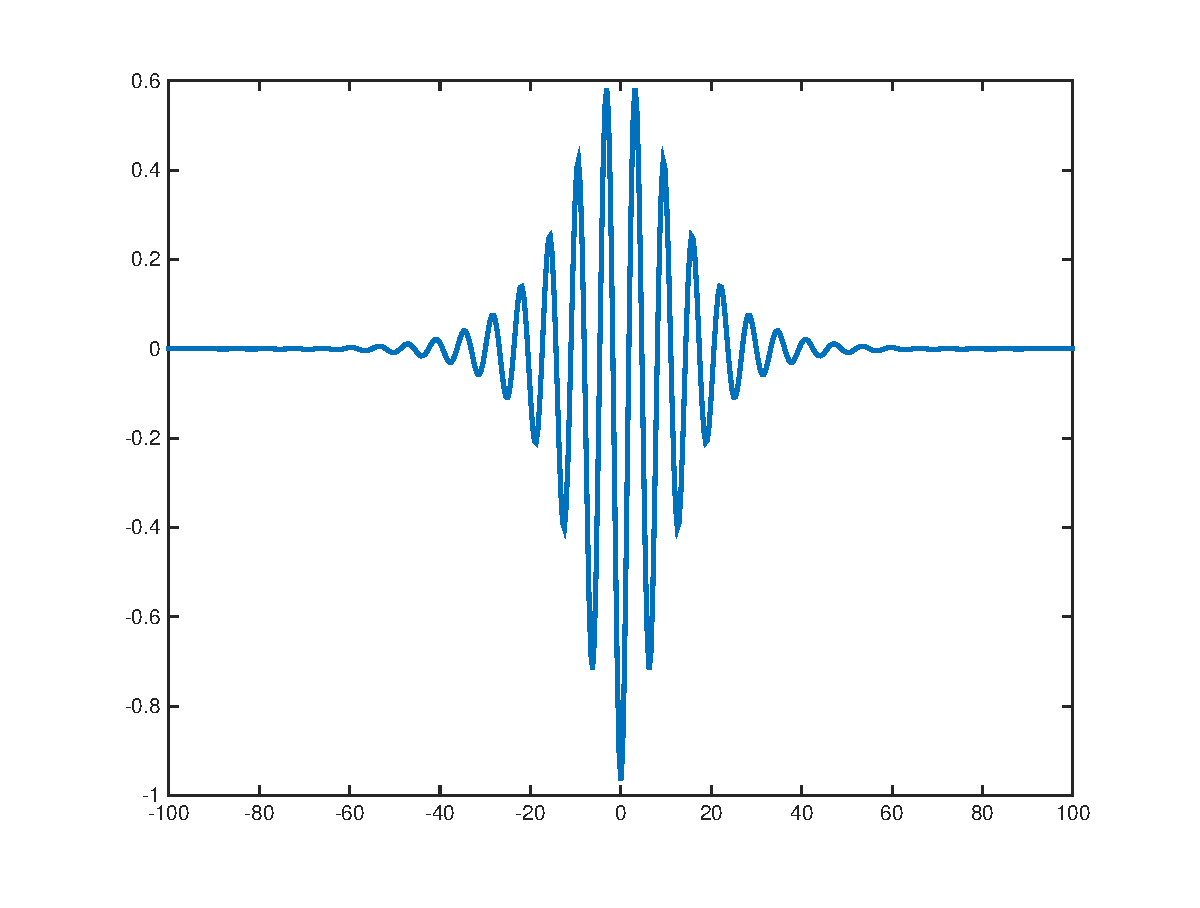
\includegraphics[width=8cm]{single14.eps}
\caption{Stationary traveling wave solutions to \eqref{eqODE}. $c = 1.354$ (left) and $c = 1.40$ (right).}
\end{figure}

We also compute solutions for other values of $c$.

\begin{figure}[H]
\centering
\includegraphics[width=8cm]{single11.eps}
\includegraphics[width=8cm]{single12.eps}
\caption{Stationary traveling wave solutions to \eqref{eqODE}. $c = 1.1$ (left) and $c = 1.2$ (right).}
\end{figure}

Let $\nu = \pm \alpha \pm i \beta$ be the eigenvalues of the linearization about the zero solution. Then we can show numerically that the tail decays exponentially with rate (approximately) $\alpha$, and the period of the tail oscillations is (approximately) $2 \pi / \beta$. This is what we expect. \\

As in the other cases, we expect that we can join the tails to form double pulses every quarter period, i.e. every $\pi / 2 \beta$. Using the same method as we always use, together with Matlab's \texttt{fsolve}, here are the first four double pulses for $c = 1.2$.

\begin{figure}[H]
\centering
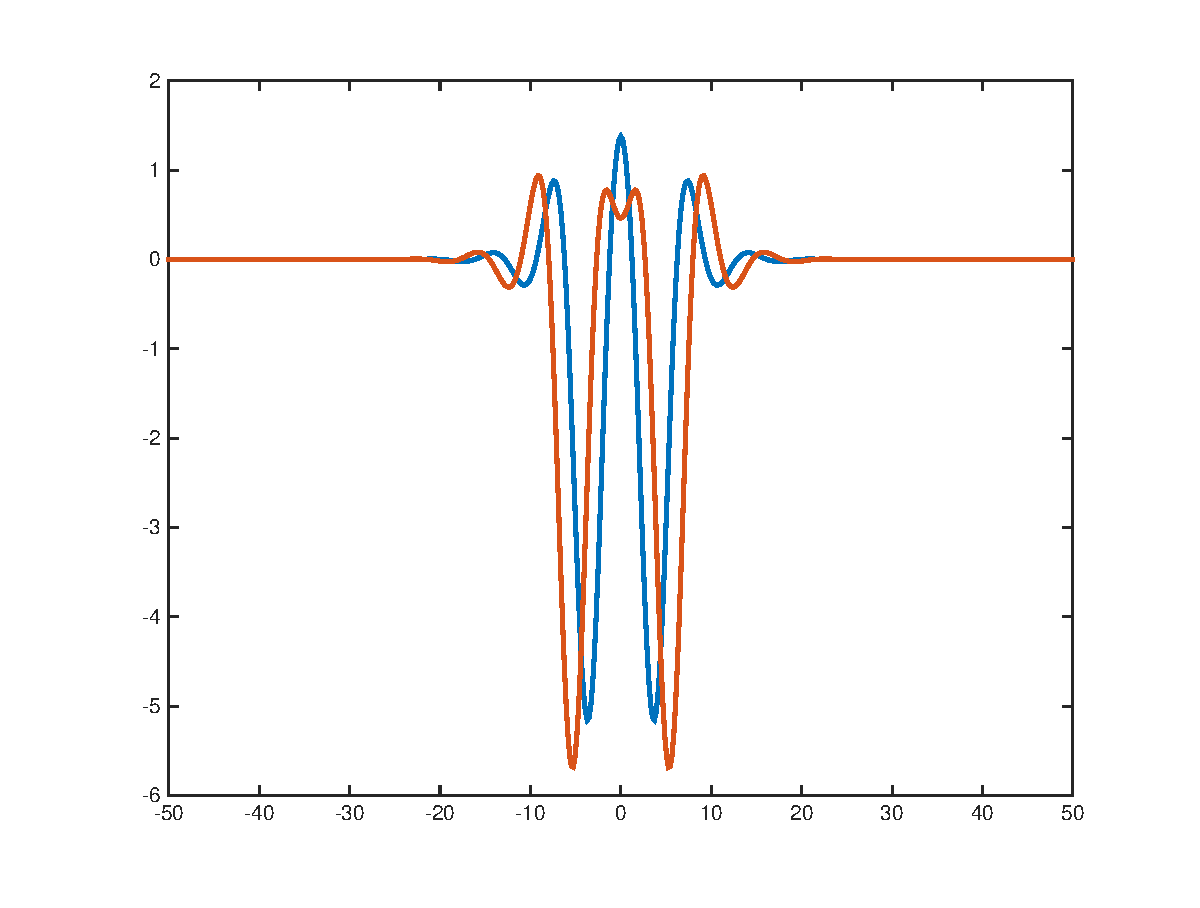
\includegraphics[width=8cm]{double12_12.eps}
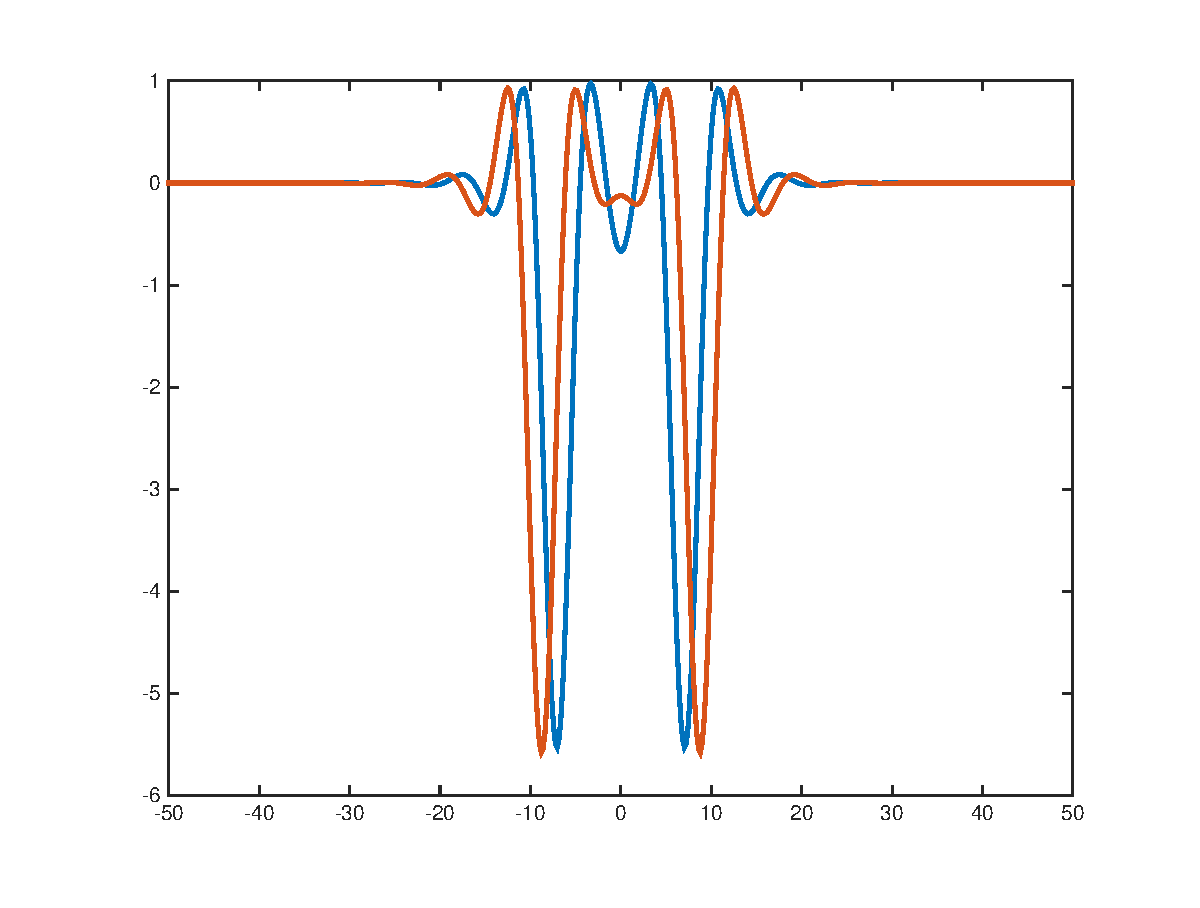
\includegraphics[width=8cm]{double12_34.eps}
\caption{Stationary double pulse traveling wave solutions to \eqref{eqODE} for $c = 1.2$. Double pulses 1 and 2 (left). Double pulses 3 and 4 (right).
\end{figure}

We can obtain periodic versions of all of these by interpolating the finite difference solutions onto the appropriate periodic grid, writing the operators using Fourier spectral matrices, and using \texttt{fsolve}.





\end{document}